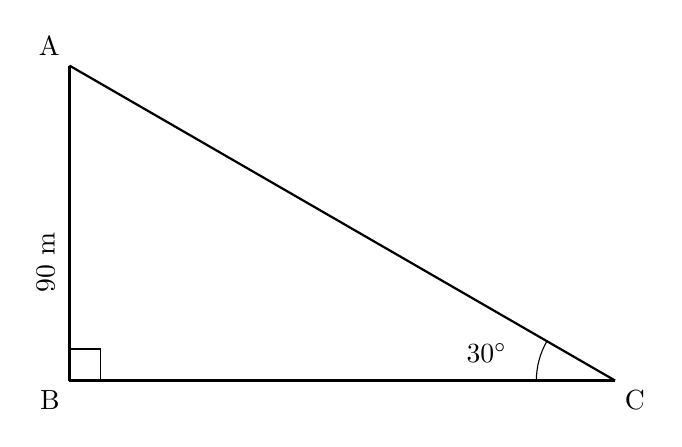
\begin{tikzpicture}

% Define the coordinates of the triangle vertices
\coordinate (B) at (0,0);
\coordinate (A) at (0,4);
\coordinate (C) at (6.93,0);

% Draw the triangle sides
% Side AB (vertical)
\draw[thick] (A) -- (B);
% Side BC (horizontal base)
\draw[thick] (B) -- (C);
% Side AC (hypotenuse)
\draw[thick] (A) -- (C);

% Draw the right angle symbol at B
\draw (B) ++(0,0.4) -- ++(0.4,0) -- ++(0,-0.4);

% Draw the angle arc at vertex C (30 degrees)
\draw (C) ++(180:1) arc (180:150:1);

% Label the vertices
\node[above left] at (A) {A};
\node[below left] at (B) {B};
\node[below right] at (C) {C};

% Label the angle at C (30 degrees)
\node at (5.3,0.35) {$30^{\circ}$};

% Label the side AB with "90 m" (rotated to be along the side)
\node[left, rotate=90] at (-0.3,2) {90 m};

\end{tikzpicture}